\chapter{Configurando GWT para funcionar com o MDArte}
\label{gwt-config}
Neste apêndice veremos um exemplo de como configurar uma aplicação GWT para acessar os serviços de um projeto MDArte. É assumido
que o leitor já tenha feito todo tutorial e que tenha dominínio da língua inglesa.

Antes de começar, existem quatro pastas zipadas que é recomendável baixar:

\begin{itemize}
  \item SistemaAcademico.zip (aplicação MDArte já pronta com o login entre ela
  e a aplicação GWT já configurada)
  \item SistemaAcademicoGWT.zip (aplicação GWT pronta para ser utilizada)
  \item SistemaAcademicoEAR.zip (aplicação EAR já configurada)
  \item jboss.zip (servidor JBOSS já configurado)
\end{itemize}

Neste tutorial, será mostrado como configurar a aplicação MDArte para habilitar a aplicação GWT a fazer login e acessar os
serviços. Em seguida, ferramentas e conceitos utilizados no desenvolvimento da aplicação GWT serão apresentados. Também serão
apresentadas a criação de uma aplicação EAR, realização do deploy dela no servidor JBoss e o funcionamento dela. Finalmente, os
passos necessários para executar a aplicação GWT serão descritos. Caso você queira

\section{Configurando a aplicação MDArte}

Nosso objetivo é que a aplicação GWT tenha acesso as serviços da aplicação MDArte. Não é necessária nenhuma configuração se a
aplicação GWT apenas utilizar serviços públicos mas se tiver que utilizar algum serviço privado que requer login será necessário
fazer alterações na classe \texttt{ControleAcessoImpl.java}. Adicione as seguintes funções:

\begin{framed}
\begin{lstlisting}[language=java, breaklines=true]
	public Subject login (String login, String senha) {

		LoginContext loginCtx = null;

		try{
			
			CallbackHandler handler = new LoginCallbackHandler(login, senha);
			loginCtx = new LoginContext("SistemaAcademico", handler);
			loginCtx.login();
			Subject subject = loginCtx.getSubject();
			accessControl.SecurityHolder.setSubject(subject);
			PrincipalImpl principal = getCallerPrincipal(subject);
			principal.setNomeProjeto("SistemaAcademico");

			return subject;
		}catch (LoginException le){
			
			System.out.println(le.getMessage());
			return null;
		}
	}
	
	public void quitLogin() {
		accessControl.SecurityHolder.setSubject(null);
	}
	
	public boolean isLogged() {
		if (accessControl.SecurityHolder.getSubject() != null) return true;
		return false;
	}
\end{lstlisting}
\end{framed}

A função \texttt{login} retorna um \texttt{Subject} que é um objeto que contém as informações de acesso do usuário. É por conta do
usuário o que ele fará com este objeto. Caso o \texttt{login} falhe um \texttt{null} será retornado.

A função \texttt{quitLogin} faz com que o Controle de Acesso não tenha mais o \texttt{Subject} impossibilitando o acesso a
serviços privados.

A função \texttt{isLogged} checa se o usuário da sessão está logado.

\section{Aplicação GWT}

\subsection{O que é GWT e onde faço download?}

GWT (Google Web Tookit) é um framework open source de desenvolvimento para construir e otimizar aplicações complexas baseadas em
browsers. O objetivo dele é permitir o desenvolvimento produtivo de aplicações web de alta performance sem que o desenvolvedor
seja um expert em particularidades de browsers \texttt{XMLHttpRequest}, and \texttt{JavaScript}.

Para fazer download vá para \texttt{http://www.gwtproject.org/download.html}.
Faça download do GWT SDK e do plugin do Eclipse. Para instalar o plugin siga as
instruções em \texttt{http://www.gwtproject.org/usingeclipse.html}.

\subsection{O que é mvp4g e onde faço download?}

Mvp4g é um framework que ajuda o desenvolvedor a construir aplicações GWT seguindo as melhores práticas segundo o padrão MVP
(Model View Presenter). O mvp4g oferece uma solução para seguir as melhores práticas usando mecanismos simples que necessitam de
poucas linhas de código e algumas anotações.

Para fazer download do mvp4g vá para \texttt{https://code.google.com/p/mvp4g/}.
Para integrar o mvp4g com uma aplicação GWT siga as instruções em
\texttt{https://code.google.com/p/mvp4g/wiki/HowtoIntegrateMvp4g}

\subsection{Criando uma aplicação GWT}

Descompacte o GWT SDK que você fez download. No terminal vá para a pasta do GWT descompactada e execute o seguinte comando.

\texttt{./webAppCreator -out SistemaAcademicoGWT br.mdarte.exemplo.academico.SistemaAcademicoGWT}

O primeiro argumento é o nome do projeto e o segundo é o pacote padrão do projeto. Na pasta raiz do projeto gerado copie o arquivo
\texttt{build.xml}.

Em seguida crie um novo projeto do tipo \texttt{Web Application Project} no Eclipse.

\begin{figure}[H]
	\centering
	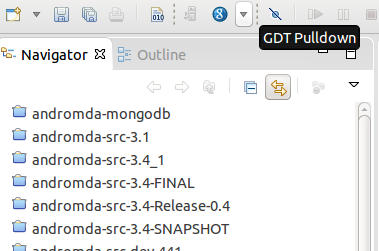
\includegraphics[scale=0.8]{files/imgs/gwt-00.png}
	\caption{Acessando o menu do plugin do GWT.}
	\label{gwt00}
\end{figure}

Um menu aparecerá ao clicar o botão a esquerda de \texttt{GDT Pulldown}na imagem acima.Clique em \texttt{New Web Application
Project\ldots}

\begin{figure}[H]
	\centering
	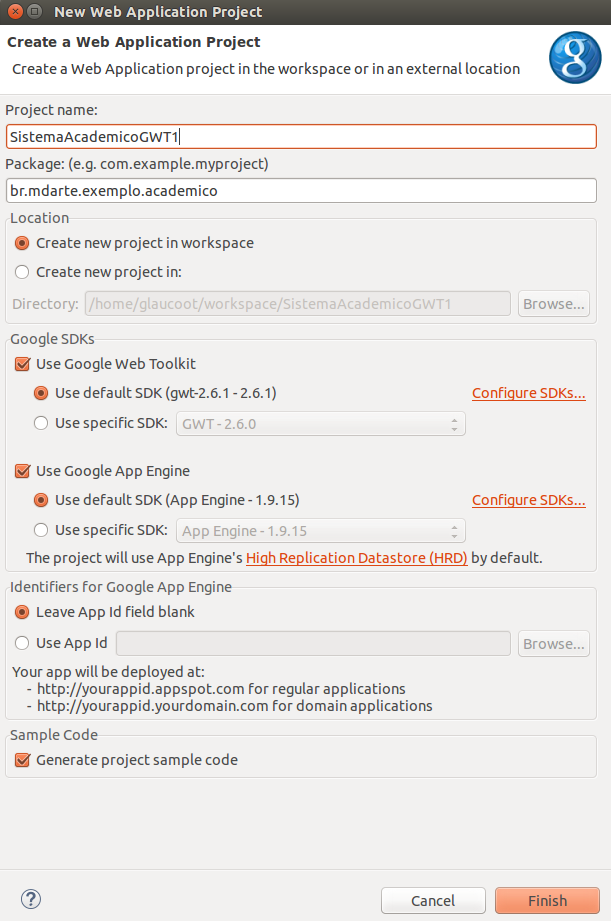
\includegraphics[scale=0.5]{files/imgs/gwt-01.png}
	\caption{Criando um novo projeto GWT no Eclipse.}
	\label{gwt01}
\end{figure}

Coloque o nome e o pacote iguais ao do projeto criado pelo terminal. Em seguida clique no primeiro \texttt{Configure SDKs\ldots},
a seguinte tela aparecerá:

\begin{figure}[H]
	\centering
	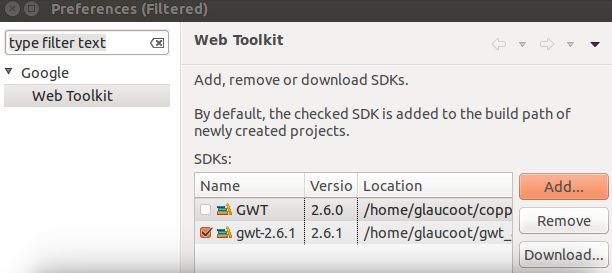
\includegraphics[scale=0.5]{files/imgs/gwt-02.png}
	\caption{Selecionando a versão do GWT que o projeto Eclipse usará}
	\label{gwt02}
\end{figure}

Nesta tela você seleciona a versão do GWT que os projetos GWT criados no Eclipse usarão. Esse passo é necessário devido ao fato da
versão do GWT que vem com o plugin do Eclipse não ser a mais atual. Clique em \texttt{Add\ldots}:

\begin{figure}[H]
	\centering
	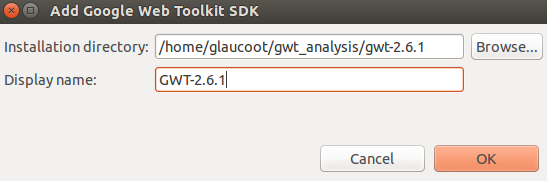
\includegraphics[scale=0.6=5]{files/imgs/gwt-03.png}
	\caption{Indicando ao caminho da nova versão GWT que o projeto usará}
	\label{gwt03}
\end{figure}

No \texttt{Installation directory} indique onde o caminho da pasta do GWT que você descompactou. De preferência, coloque no
\texttt{Display Name} a versão do GWT. Após clicar em OK, marque o SDK recentemente criado como na figura anterior.

Com o projeto criado, passe o \texttt{build.xml} que você copiou para o projeto do Eclipse. Passe os JARS indicados por
\texttt{https://code.google.com/p/mvp4g/wiki/HowtoIntegrateMvp4g} para a pasta
\texttt{/war/WEB-INF/lib}. A lista de jars que tem que ser obtidos é a seguinte:

\begin{itemize}
  \item aopalliance.jar
  \item gin-2.1.2.jar
  \item guice-3.0.jar
  \item guice-assistedinject-3.0.jar
  \item javax.inject.jar
  \item mvp-1.5.0.jar
\end{itemize}

Além disso, caso o seu projeto GWT tenha o JAR \texttt{gwt-servlet-deps.jar} remova-o. Agora você tem um projeto GWT com as
dependências necessárias instaladas.

\section{Aplicação EAR}

EAR (Enterprise ARchive) é um JAR com extensão \texttt{.ear} usado no Java EE para empacotar um ou mais módulos em um único
arquivo para que o \texttt{deploy} de vários módulos em um servidor de aplicação aconteçam simultaneamente e coerentemente.

Utilizamos esse tipo de arquivo para transformar a aplicação MDArte e o Controle de Acesso em módulos que a aplicação GWT possa
acessar os serviços dessas aplicações. Vale notar que a aplicação GWT não terá acesso a funcionalidade web de seus módulos pois o
EAR só comportar um arquivo EAR.

\subsection{Criando uma aplicação EAR}

No Eclipse, clique no botão \texttt{New}. A seguinte tela aparecerá:

\begin{figure}[H]
	\centering
	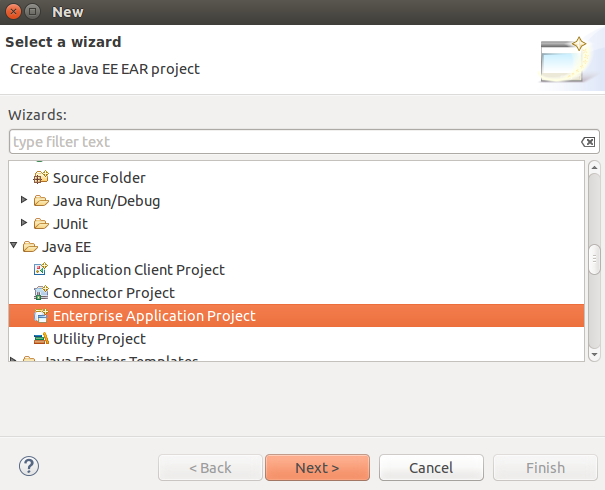
\includegraphics[scale=0.5]{files/imgs/gwt-04.png}
	\caption{Criando um projeto EAR}
	\label{gwt04}
\end{figure}

Selecione \texttt{Enterprise Application Project}. A seguinte tela aparecerá:

\begin{figure}[H]
	\centering
	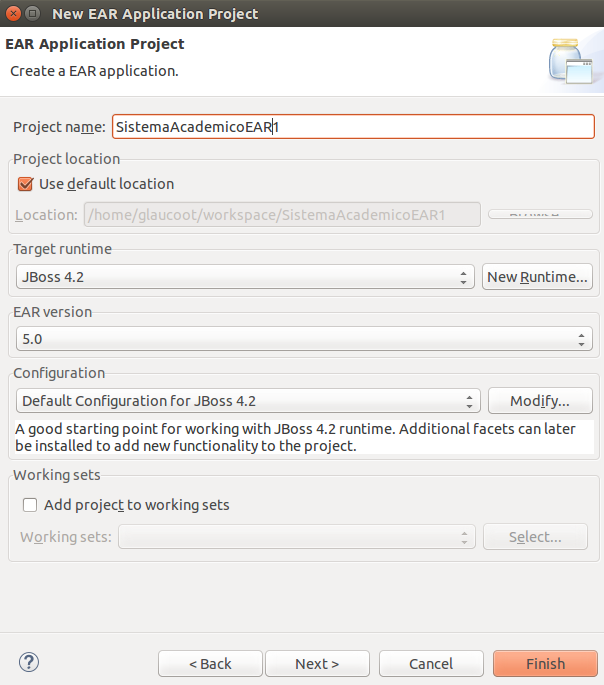
\includegraphics[scale=0.5]{files/imgs/gwt-05.png}
	\caption{Selecione o nome do projeto EAR e o tipo de servidor}
	\label{gwt05}
\end{figure}

Escolha um nome para a aplicação EAR e o tipo de servidor em que será executado. Clique em \texttt{Next>}.

\begin{figure}[H]
	\centering
	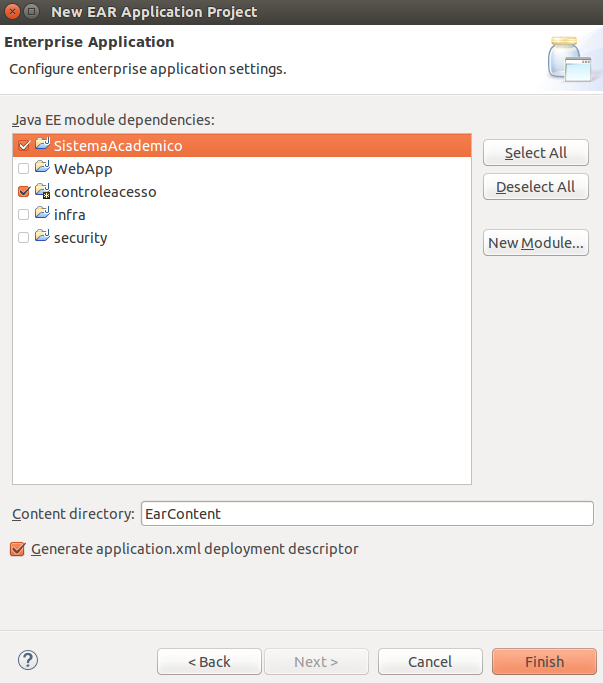
\includegraphics[scale=0.5]{files/imgs/gwt-06.png}
	\caption{Escolhendo os módulos JAR da aplicação EAR}
	\label{gwt06}
\end{figure}

Nesta tela você escolhe as aplicações que você deseja acessar os serviços. Selecione a aplicação MDArte e o Controle de Acesso.
Marque a caxinha do \texttt{Generate application.xml}. Agora temos que colocar um WAR no EAR, isso seria criar um WAR a partir da
aplicação GWT.

\subsection{Configurando a aplicação GWT para ser um WAR do EAR}

Clique com o botão direito do mouse no sua aplicação GWT e selecione \texttt{Properties}.

\begin{figure}[H]
	\centering
	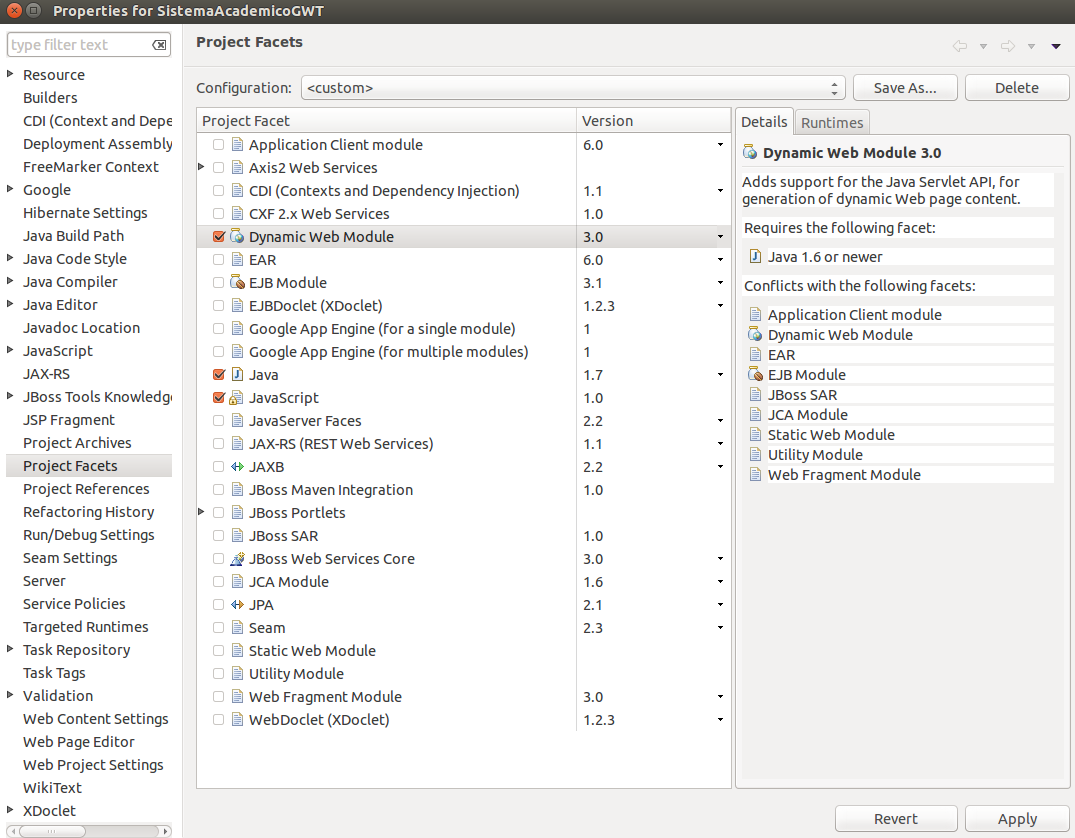
\includegraphics[scale=0.4]{files/imgs/gwt-07.png}
	\caption{Configurando a aplicação GWT para ser um WAR do EAR}
	\label{gwt07}
\end{figure}

Selecione \texttt{Project Facets}. Marque a caixa \texttt{Dynamic Web Module}. Caso o Eclipse exiba a mensagem \texttt{Cannot
change version of project version\ldots}, mude para uma versão com numeração maior clicando no \texttt{List Box} que exibe o
número da versão. Com tudo OK, clique em \texttt{Apply} e depois em OK.

\subsection{Adicionando a aplicação GWT ao EAR}

Clique com o botão direito do mouse no sua aplicação EAR e selecione \texttt{Properties}. Selecione \texttt{Deployment Assembly} e
clique \texttt{Add\ldots}. Siga as figuras:

\begin{figure}[H]
	\centering
	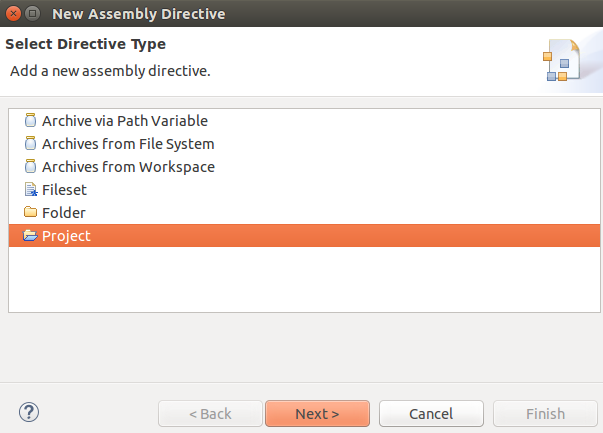
\includegraphics[scale=0.5]{files/imgs/gwt-08.png}
	\caption{Selecione um projeto do seu Workspace}
	\label{gwt08}
\end{figure}

\begin{figure}[H]
	\centering
	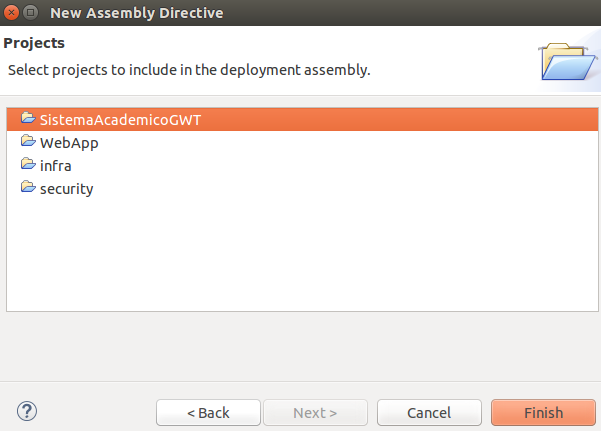
\includegraphics[scale=0.5]{files/imgs/gwt-09.png}
	\caption{Selecione a aplicação GWT}
	\label{gwt09}
\end{figure}

\begin{figure}[H]
	\centering
	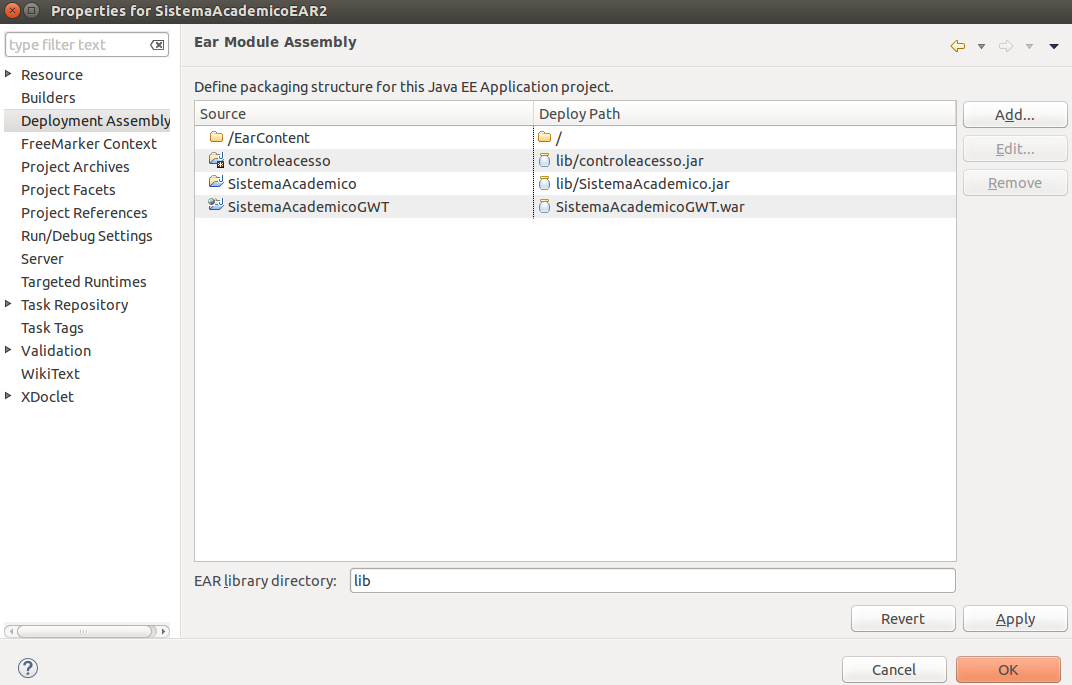
\includegraphics[scale=0.4]{files/imgs/gwt-10.png}
	\caption{Módulos da aplicação EAR}
	\label{gwt10}
\end{figure}

Clique em \texttt{Apply} e depois em OK. Agora a sua aplicação EAR está totalmente configurada.

\section{Configuração do JBoss}
Simplesmente siga as instruções do Apêndice 01 tomando o cuidado de configurar
os arquivos com o endereço dos bancos de dados que serão usados. A diferença é
que o login do GWT será feito pelo controleacesso (a configuração de login que
importa é do controleacesso).

Caso você queira executar o EAR a partir do Eclipse. Vá para a aba Servers:

\begin{figure}[H]
	\centering
	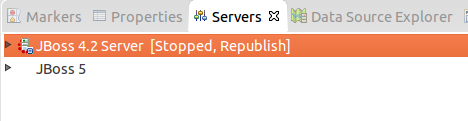
\includegraphics[scale=0.4]{files/imgs/gwt-11.png}
	\caption{Selecione o servidor que será usado}
	\label{gwt11}
\end{figure}

Selecione o servidor que será usado, clique com o botão direito do mouse e selecione \texttt{Add and Remove\ldots}

\begin{figure}[H]
	\centering
	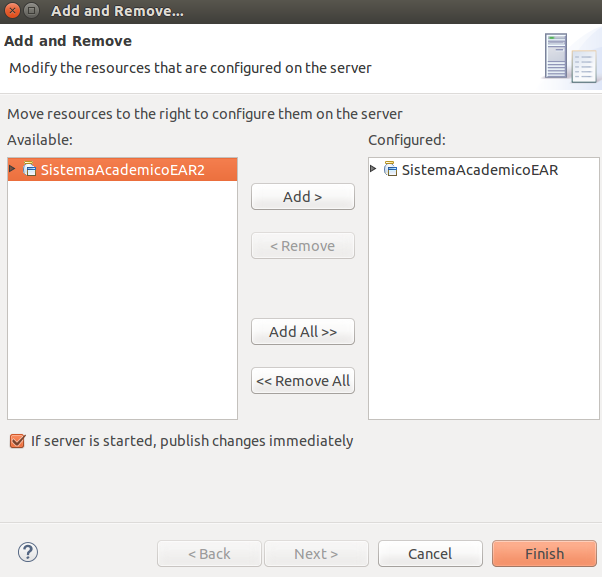
\includegraphics[scale=0.4]{files/imgs/gwt-12.png}
	\caption{Configurando o EAR}
	\label{gwt12}
\end{figure}

Clique no projeto EAR desejado, clique \texttt{Add>} e depois \texttt{Finish}

\section{Importanto os exemplos prontos}

Caso você queira usar os exemplos disponíveis em \ldots\ldots\ldots\ldots Importe os projetos no Eclipse na seguinte ordem:

\begin{itemize}
  \item SistemaAcademico
  \item SistemaAcademicoGWT
  \item SistemaAcademicoEAR
\end{itemize}

E substitua o servidor JBoss pelo da pasta jboss.zip.

É altamente recomendável que você teste e analise o código do SistemaAcademicoGWT oferecido para você ter uma idéia de como o GWT
e o mvp4g funcionam.

\section{Compilando os projetos}

Esta seção tanto serve para projetos que você próprio fez quanto para os exemplos fornecidos. Vale ressaltar que foi executado
maven clean nos projetos para reduzir o tamanho deles para download. 

Execute os seguintes comandos no terminal para averiguar se a compilação do GWT vai funcionar:

\begin{itemize}
  \item Execute \texttt{./mavex.sh -a} no pasta do \texttt{controleacesso} para dar o deploy dele no servidor e gerar os arquivos
  Java dele
  \item Execute \texttt{maven install deploy} no pasta do \texttt{SistemaAcademico} para dar o deploy dele no servidor e gerar os
  arquivos Java dele
  \item Execute Refresh nos \texttt{SistemaAcademico} e \texttt{SistemaAcademicoGWT} no Eclipse e dê Build Project no
  \texttt{SistemaAcademicoEAR} no Eclipse.
  \item Execute \texttt{ant war} na pasta do \texttt{SistemaAcademicoGWT} ou \texttt{GWT Compile} no Eclipse, a compilação tem que
  ser um sucesso.
  Assim teremos o \texttt{SistemaAcademicoGWT.war} gerado.
\end{itemize}

\section{Executando a aplicação GWT}

Passo 1: Sempre que modificar a aplicação GWT ou MDArte faça o Refresh delas e execute Build Project no
\texttt{SistemaAcademicoEAR} no Eclipse.

Passo 2: Se você modificou a aplicação MDArte ao modificar o modelo ou algum arquivo Java, execute o \texttt{maven install deploy}
ou \texttt{./mavex.sh -a} (caso disponível) nele.
Vá para o passo 1.

Passo 3: Execute \texttt{ant war} no Terminal em \texttt{SistemaAcademicoGWT} ou \texttt{GWT Compile} no Eclipse.
Caso apareça um erro de compilação tipo \texttt{cannot find symbol}, é por causa que ele não acha classes do SistemaAcademico.
Repita o Passo 1

Caso a compilação seja um sucesso, a partir deste ponto há duas formas de executar a aplicação GWT através do EAR.

\subsubsection{Executando através do Eclipse}

Passo 3a: Caso você tenha executado \texttt{ant war} no Terminal, um arquivo SistemaAcademicoGWT.war será gerado na raiz do
projeto.

Passo 4a: Coloque o \texttt{SistemaAcademicoGWT.war} no \texttt{<JBOSS\_HOME>/server/default/deploy/}.

Passo 5a: No Eclipse, clique com botão direito no projeto \texttt{SistemaAcademicoEAR} clique com o botão direito do mouse,
selecione Run As, Run on Server.

\begin{figure}[H]
	\centering
	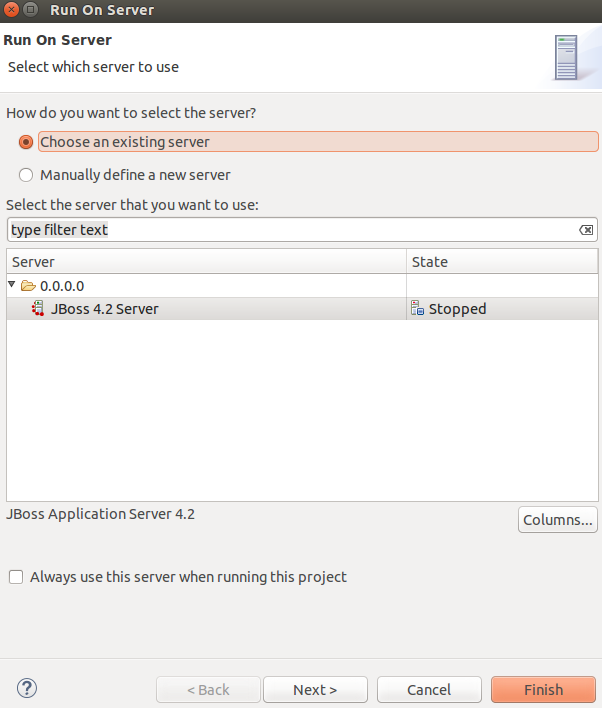
\includegraphics[scale=0.4]{files/imgs/gwt-13.png}
	\caption{Executando o EAR através do Eclipse}
	\label{gwt13}
\end{figure}

Selecione a opção \texttt{Choose an existing Server}, selecione o servidor JBoss que você criou e clique em \texttt{Finish}.

Final: A aplicação será aberta dentro do próprio Eclipse.

\subsubsection{Executando através do deploy do EAR no JBoss}

Passo 3b: Clique com o botão direito do mouse no projeto EAR e selecione \texttt{Export\ldots}

\begin{figure}[H]
	\centering
	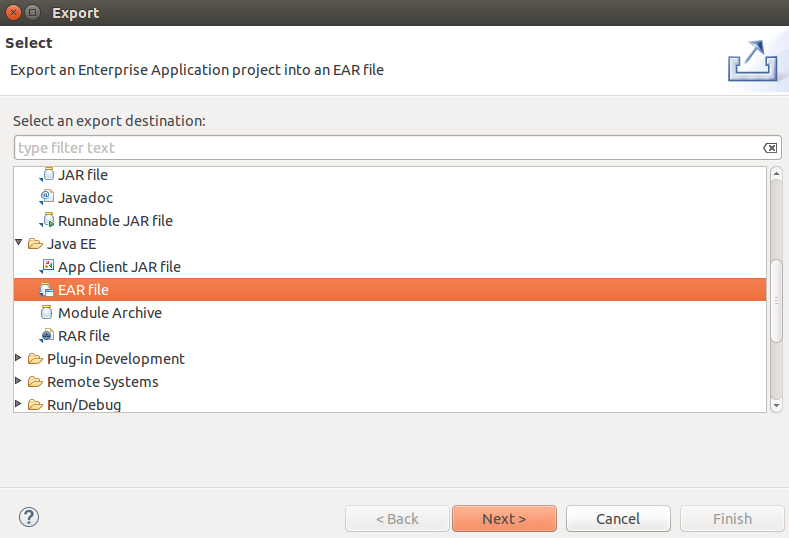
\includegraphics[scale=0.5]{files/imgs/gwt-14.png}
	\caption{Fazendo o deploy do projeto EAR}
	\label{gwt14}
\end{figure}

Passo 4b: Selecione na pasta \texttt{Java EE} a opção \texttt{EAR File}. Clique em \texttt{Next>}.

\begin{figure}[H]
	\centering
	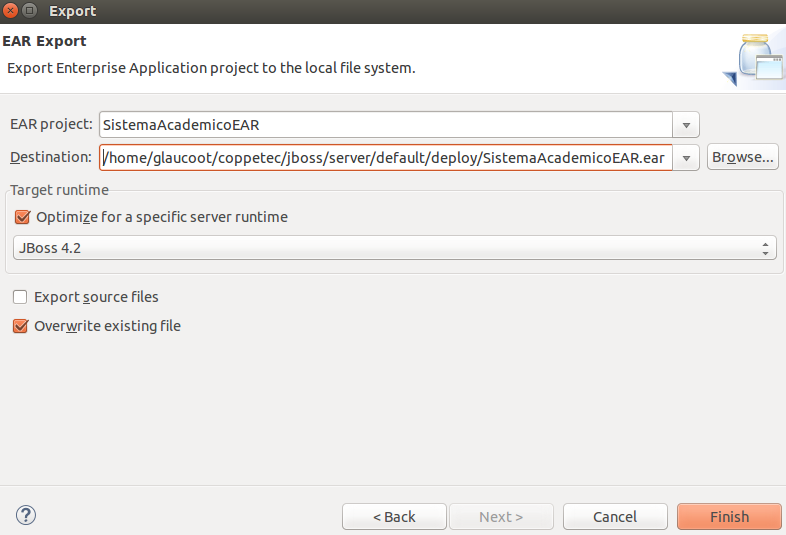
\includegraphics[scale=0.5]{files/imgs/gwt-15.png}
	\caption{Gerando o EAR na pasta do JBoss}
	\label{gwt15}
\end{figure}

Passo 5b: Em \texttt{Destination} coloque como caminho o \texttt{<JBOSS\_HOME>/server/default/deploy/}. Marque as caixas que estão
marcadas na figuras. Clique em \texttt{Finish}

Final: Pronto o arquivo EAR está no JBoss pronto para ser utilizado. Agora é só inicializar o servidor como você faz para utilizar
aplicações MDArte.

\section{Considerações finais}

A segunda forma é melhor pois você pode pegar o EAR e colocar em outro JBoss na pasta \texttt{deploy}. Você precisará dos jars
gerados da aplicação MDArte e do Controle de Acesso também. Os arquivos WAR não são necessários para o funcionamento do EAR.

Outro ponto importante, é que ao executar todos esses passos não será possível executar a aplicação GWT em Super Dev mode.


\section{Configurando o build path (Opcional)}

Tenha pelos menos as variáveis MAVEN\_REPO e JBOSS\_HOME configuradas no \texttt{build path} do seu Eclipse. Ter essas duas
variáveis será uma grande ajuda durante o desenvolvimento dos seus projetos. O Eclipse fará o auto complete para você de funções de bibliotecas
do repositório e imports automáticos além de apontar em erros de codificação sem você precisar compilar o código.

Se não tiver elas no \texttt{build path}, MAVEN\_REPO tem que apontar para a pasta .maven da sua máquina que seria
\texttt{<HOME>/.maven/repository}. JBOSS\_HOME deve apontar para a mesma pasta da variável de ambiente \$JBOSS\_HOME que foi
configurada no início do tutorial.

Para criar a variável MAVEN\_REPO e JBOSS\_HOME, clique com o botao direito em qualquer projeto Java e selecione Properties.

Selecione Java Built Path -> Selecione Add Variable... -> Selecione Configure Variables... -> Selecione New... -> Ponha o nome e o path desejados.

\section{Referências}

http://jamies-gwt.blogspot.com.br/2010/03/walkthrough-integrating-gwt-with-jboss.html

http://www.gwtproject.org/

https://code.google.com/p/mvp4g/

http://samples.gwtproject.org/samples/Showcase/Showcase.html
